\section{Patterns 6 - Redegør for følgende concurrency mønstre}

\subsection{Fokuspunkter}

\begin{itemize}
	\item Parallel Loops.
	\item Parallel Tasks.
\end{itemize}

\subsection{Task Parallel Library}
\begin{itemize}
	\item Bibliotek i .NET.
	\item Man behøver ikke vide hvor mange kerner programmet skal køre på.
	\begin{itemize}
		\item På general-purpose platforme kan programmøren ikke forudsige hvor mange kerne/hvilken hardware der er til rådighed.
	\end{itemize}
	\item TPL sørger for Dynamisk Load Balancing.
	\item Der er ikke garenti for hvilken rækkefølge tasks afvikles i. 
\end{itemize}

\subsection{Parallel loops}

Parallel loops pattern minder meget om et almindeligt loop. Der udføres samme operation hvor hvert element for et givet antal gange. Forskellen er dog at et almindeligt loop sker sekventielt, hvorimod et parallelt loop ofte udfører steps parallelt. Når man bruger parallelle loops er det derfor vigtigt at sikre sig at iterationerne ikke er afhængige af hinanden.

Eksempel på almindeligt for loop:

\begin{lstlisting}[caption=Normal for loop, label=code:normalLoop]
for (int i = 0; i < n; i++)
{
	//Do stuff...
}
\end{lstlisting}

Eksempel på parallelt for loop: lambda expression

\begin{lstlisting}[caption=Parallel for loop,  label=code:paraLoop,
morekeywords={Parallel, For}]
Parallel.For (0, n, i =>
{
	//Do stuff...
});
\end{lstlisting}

For Each løkken kan også køres parallelt: lambda expression

\begin{lstlisting}[caption=Parallelt for each loop, label=paraForEach,morekeywords={string,Parallel, ForEach, WriteLine}]
string[] navne = { "Torben", "Birger", "Niels" };

Parallel.ForEach(navne, navn =>
{
	Console.WriteLine(navn);
});
\end{lstlisting}

Det er Task Parallel Library der står for at håndtere threading, og man skal derfor ikke selv sørge for at fordele opgaven til CPU'en. 

\subsubsection{Hvornår giver det mening med Parallel Loops?}
\begin{itemize}
	\item Som sagt kan det kun bruges hvor iterationerne ikke er afhængige af hinanden!
	\item Brug når iterationer ikke tilgår samme memory/filer.
	\item Brugbart hvor der laves blokerende kald (skriv/læs til fil).
	\item Brugbart når beregninger kan spredes ud på flere kerner.
\end{itemize}

Trådhåndtering giver overhead på et parallelt loop, og derfor kan meget små iteraationer blive kvalt heri.

TPL håndterer partitionering, thread scheduling af tråde i threadPool'en og generelt alle low-level details.

\subsection{Parallel tasks}

En task er ikke en tråd! En task er en opgave som udføres \textbf{sekventielt}.\\

Vi kan bruge \textbf{Task Parallel Library} biblioteket til at køre disse tasks parallelt. TPL kan selv dynamisk scale graden af parallelisme sådan at det mest effektict udnytter de kerner den har til rådighed.

\subsection{Thread Pool}
Måde at ''opbevare'' flere tasks, sådan at en færdig tråd altid kan hente nye opgaver.

\subsubsection{Den simpel og dårlige løsning}
Den simple \textbf{og dårlige(!)} løsning, som ikke benyttes af TPL. 

\begin{figure}[h]
	\centering
	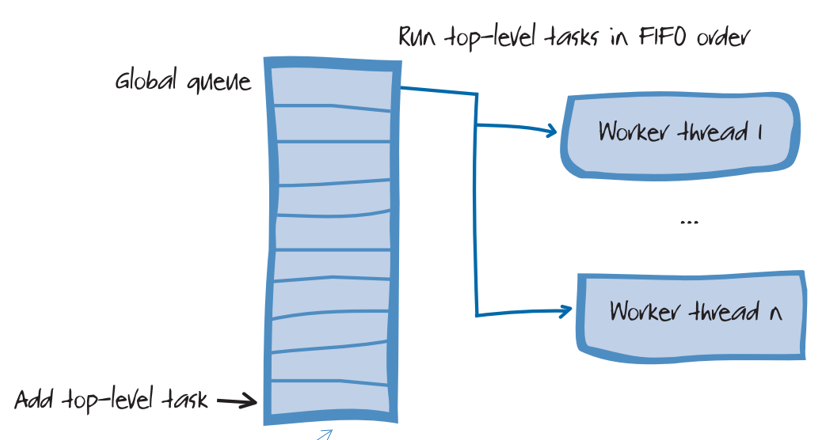
\includegraphics[width=0.7\linewidth]{figs/badthreadpool}
	\caption{Simple implementering af threadpool}
	\label{fig:badthreadpool}
\end{figure}


\begin{itemize}
	\item Naiv og langsom.
	\item Én global kø, som alle tråde henter jobs fra.
	\item Betyder at kun én tråd kan hente et job af gangen.
	\begin{itemize}
		\item Køen bliver flaskehalsen.
		\item Mange små tasks forværre problemet.
		\item Køen bliver tilgået ofte, giver stort overhead.
	\end{itemize}
\end{itemize}

\subsubsection{Den gode}

\begin{figure}[h]
	\centering
	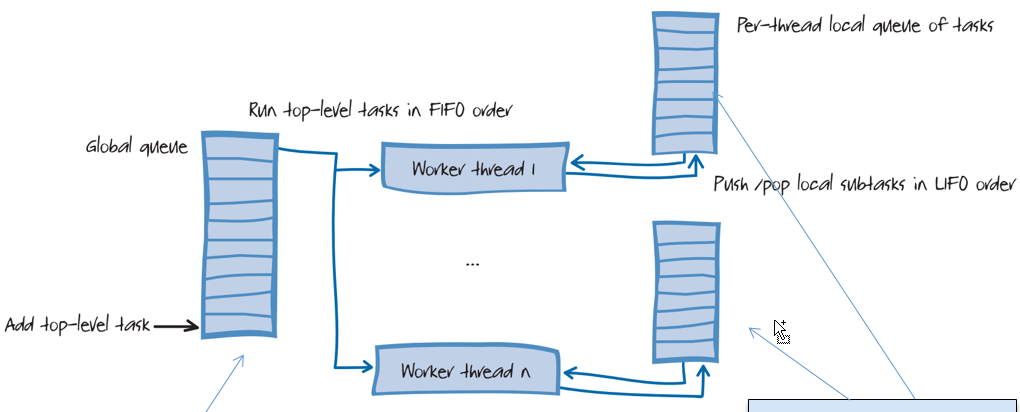
\includegraphics[width=\linewidth]{figs/goodthreadpool}
	\caption{Faktisk implementering af threadpool, i .NET.}
	\label{fig:goodthreadpool}
\end{figure}

\begin{itemize}
	\item En global kø.
	\begin{itemize}
		\item Opbevare tasks som endnu ikke er delt ud på en tråd.
	\end{itemize}
	\item Hver tråd har sin egen kø.
	\begin{itemize}
		\item Tråde skal ikke vente på synkronisering med den globale kø.
		\item Er LIFO i begge ender.
		\item Har en privat og offentlig ende.
		\item Når køen er tom, hentes tasks fra den globale kø.
	\end{itemize}
	\item Work stealing.
	\begin{itemize}
		\item Tråde kan ''stjæle'' hinandens tasks.
		\item Det sker når egen og global kø er tomme.
		\item Tråde tilgår kun den offentlige ende af andres køer.
	\end{itemize}
	\item Inline execution
	\begin{itemize}
		\item hvis...
		\begin{itemize}
			\item \textit{task1} venter på \textit{task2}.
			\item \textit{task2} er ikke startet når \textit{task1} venter.
			\item Begge tasks er placeret i samme kø.
		\end{itemize}
		\item ... kan scheduleren.
		\begin{itemize}
			\item Give \textit{task2} højere prioritet og afvikle den med samme.
			\item Så \textit{task1} bliver hurtigere færdig.
		\end{itemize}
	\end{itemize}
\end{itemize}

\subsection{Kodeeksempler}

I kode udsnit~\ref{code:tasknormal} udføres en opgave på gammel sekventiel vis, mens listing~\ref{code:taskparallel} viser bruges af \textit{Parallel.Invoke()}.

\begin{lstlisting}[
caption=Almindelig udførsel af opgave.,
label=code:tasknormal]
// Old sequencial way of doing things
public void DoAll() {
	DoLeft();
	DoRight();
}
\end{lstlisting}

\subsubsection{Invoke}
I eksemplet eksisterer to funktioner: DoLeft() og DoRight(). De to funktioner bliver afviklet asynkront vha. TPL. Dette er den mest simple måde at starte tasks på.\\

Invoke-metoden returnerer når alle tasks er afviklet.
\begin{lstlisting}[
caption=Parallel udførsel af opgave/task.,
label=code:taskparallel,
morekeywords={Parallel, Invoke}]
// Simplest start af threads, vha invoke
public void DoAll() {
	Parallel.Invoke(DoLeft, DoRight); // blocks till finished
}
\end{lstlisting}

\subsubsection{StartNew, Wait og WaitAll}
Ligeledes kan funktionerne \textit{DoRight()} og \textit{DoLeft()} udføres med TaskFactory som i listing~\ref{code:taskfactory}.

\begin{lstlisting}[
caption=Brug af TaskFactory - gør det samme som listing~\ref{code:taskparallel},
label=code:taskfactory,
morekeywords={Task, Factory, StartNew, Wait, WaitAll}]
public void DoAll() {
	Task t1 = Task.Factory.StartNew(DoLeft);
	Task t2 = Task.Factory.StartNew(DoRight);
	
	// Enten det her...
	Task.WaitAll(t1, t2);
	
	// Eller det her
	t1.Wait();
	t2.Wait();
}
\end{lstlisting}

\subsubsection{WaitAny}
\textit{WaitAny()} afventer, at mindst én task er blevet afviklet. Det kan benyttes til at udføre arbejde, mens der stadig ventes på, at andre tasks er blevet afviklet færdigt.

\todo{forstår ikke helt linje 14 i det nedenstående..}
\begin{lstlisting}[
caption=Brug af WaitAny.,
label=code:taskfactory,
morekeywords={Task, Factory, StartNew, Wait, WaitAll}]
Task[] tasks = {
	Task.Factory.StartNew(DoLeft),
	Task.Factory.StartNew(DoCenter),
	Task.Factory.StartNew(DoRight),
};

while(tasks.Length > 0) {
	var taskIndex = Task.WaitAny(tasks);
	
	// Do meaningful work with task[taskIndex] here.
	
	// Update the set of tasks upon which we wait.
	// Filter out the completed task (remove it from tasks-array).
	tasks = tasks.Where((t) => t != tasks[taskIndex]).ToArray();
}
\end{lstlisting}

\subsubsection{Giv en variable med til en \textit{task}}
I eksemplet startes 4 tasks, som hver især udskriver deres index (0-3).\\

\textit{i} kan ikke benyttes direkte i lambda-udtrykket, da den er global mellem alle fire tasks. Inden den første task går i gang med at afvikle kan i have værdien 3.

Løsning: Lav en midlertidig variabel, sæt den til at pege på i, og benyt den i stedet.

\begin{lstlisting}[
caption=Giv en tråd en variable med.,
label=code:threadvariable,
morekeywords={Task, Console, var}]
for (int i = 0; i< 4; i++)
{
	var tmp = i;
	Task.Factory.StartNew(() => Console.WriteLine(tmp));
}
\end{lstlisting}

Bemærk: Hvis der IKKE laves en midlertidig variabel, vil i være delt mellem alle tasks. Det kan i nogle tilfælde være nødvendigt.

\subsubsection{Kør en \textit{task} på et objekt}
Dette er en anden måde at give data med til en task.\\

Der afvikles en metode på et objekt. Metoden har adgang til alle attributter på objektet.

\begin{lstlisting}[
caption=Giv en tråd en variable med vha klasser.,
label=code:threadvariable2,
morekeywords={Task, Console, var, string}]
class Work
{
	public int Data1;
	public string Data2;
	public void Run()
	{
		Console.WriteLine(Data1 + ": " + Data2);
	}
}

public static void Main()
{
	Work w = new Work();
	w.Data1 = 42;
	w.Data2 = "The Answer to the Ultimate Question of ...";
	Task.Factory.StartNew(w.Run);
}
\end{lstlisting}